%coding:utf-8

%----------------------------------------
%FOSAPHY, a LaTeX-Code for a summary of mathematics
%Copyright (C) 2013, Mario Felder, Michael Fallegger

%This program is free software; you can redistribute it and/or
%modify it under the terms of the GNU General Public License
%as published by the Free Software Foundation; either version 2
%of the License, or (at your option) any later version.

%This program is distributed in the hope that it will be useful,
%but WITHOUT ANY WARRANTY; without even the implied warranty of
%MERCHANTABILITY or FITNESS FOR A PARTICULAR PURPOSE.  See the
%GNU General Public License for more details.
%----------------------------------------

\documentclass[a5paper,10pt,fleqn]{book}

\usepackage{layout}

\title{Formelsammlung Mathematik}

\author{Mario Felder\\Michi Fallegger}
\date{\today}

%\catcode `\*=\active
%\def *{\cdot}

\begin{document}

\maketitle
\thispagestyle{empty}
\cleardoublepage
\pagenumbering{Roman}
\tableofcontents
% coding:utf-8

%----------------------------------------
%FOSAPHY, a LaTeX-Code for a summary of mathematics
%Copyright (C) 2013, Mario Felder, Michael Fallegger

%This program is free software; you can redistribute it and/or
%modify it under the terms of the GNU General Public License
%as published by the Free Software Foundation; either version 2
%of the License, or (at your option) any later version.

%This program is distributed in the hope that it will be useful,
%but WITHOUT ANY WARRANTY; without even the implied warranty of
%MERCHANTABILITY or FITNESS FOR A PARTICULAR PURPOSE.  See the
%GNU General Public License for more details.
%----------------------------------------

	\setcounter{page}{1}
    \pagenumbering{arabic}
% coding:utf-8

%----------------------------------------
%FOSAPHY, a LaTeX-Code for a summary of mathematics
%Copyright (C) 2013, Mario Felder, Michael Fallegger

%This program is free software; you can redistribute it and/or
%modify it under the terms of the GNU General Public License
%as published by the Free Software Foundation; either version 2
%of the License, or (at your option) any later version.

%This program is distributed in the hope that it will be useful,
%but WITHOUT ANY WARRANTY; without even the implied warranty of
%MERCHANTABILITY or FITNESS FOR A PARTICULAR PURPOSE.  See the
%GNU General Public License for more details.
%----------------------------------------

\chapter{Repetition}
\section{Kreisgleichung}
Der Mittelpunkt des Kreises wird mit $x_0$ und $y_0$ angegeben.\\
\newline
\[
	\boxed{(x-x_{0})^2+(y-y{0})^2=r^2 }
\]	
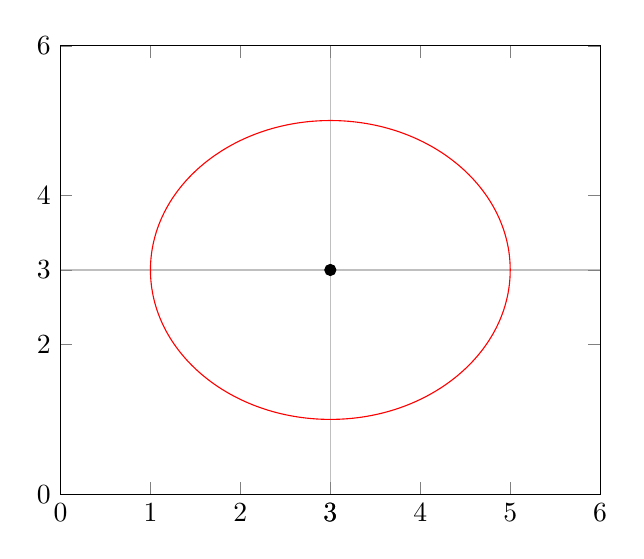
\begin{tikzpicture}
\begin{axis}[
	xmin=0,   xmax=6,
	ymin=0,   ymax=6,
	extra x ticks={3},
	extra y ticks={3},
	extra tick style={grid=major},
]
	\draw[red] \pgfextra{
	  \pgfpathellipse{\pgfplotspointaxisxy{3}{3}}
		{\pgfplotspointaxisdirectionxy{2}{0}}
		{\pgfplotspointaxisdirectionxy{0}{2}}
	  % see also the documentation of 
	  % 'axis direction cs' which
	  % allows a simpler way to draw this ellipse
	};
	\addplot [only marks,mark=*] coordinates { (3,3) };
\end{axis}
\end{tikzpicture}
\\
\\
Rotation um die z-Achse
\[
	\boxed{z=f(x,y)=g(\sqrt{x^2+y^2}}
\]
\\
\\




   
% coding:utf-8

%----------------------------------------
%FOSAPHY, a LaTeX-Code for a summary of mathematics
%Copyright (C) 2013, Mario Felder, Michael Fallegger

%This program is free software; you can redistribute it and/or
%modify it under the terms of the GNU General Public License
%as published by the Free Software Foundation; either version 2
%of the License, or (at your option) any later version.

%This program is distributed in the hope that it will be useful,
%but WITHOUT ANY WARRANTY; without even the implied warranty of
%MERCHANTABILITY or FITNESS FOR A PARTICULAR PURPOSE.  See the
%GNU General Public License for more details.
%----------------------------------------

\chapter{Partielle Ableitung}
\section{Partielle Ableitung??}
% \[v=\lim\limits_{\Delta x \to 0}{\frac{f(x_{0}+\Delta x)-f(x_{0}){\Delta x}} \approx \frac{\Delta y}{\Delta x}\]		
% coding:utf-8

%----------------------------------------
%FOSAPHY, a LaTeX-Code for a summary of mathematics
%Copyright (C) 2013, Mario Felder, Michael Fallegger

%This program is free software; you can redistribute it and/or
%modify it under the terms of the GNU General Public License
%as published by the Free Software Foundation; either version 2
%of the License, or (at your option) any later version.

%This program is distributed in the hope that it will be useful,
%but WITHOUT ANY WARRANTY; without even the implied warranty of
%MERCHANTABILITY or FITNESS FOR A PARTICULAR PURPOSE.  See the
%GNU General Public License for more details.
%----------------------------------------

\chapter{Differential Funktionen}
\section{Tangentialebene, Linearisierung, totales Differential}
Die Gleichung der Tangentialebene an die Fläche $z=f(x,y)$ im Punkt$(x_0,y_0,z_0)$, $z_0=f(x_0,y_0)$ lautet:
\[
\boxed{\begin{aligned}	
		z&=f(x_0,y_0) + f_{'x}(x_0,y_0)(x-x_0)+ f_{'y}(x_0,y_0)(y-y_0)
	\end{aligned}}\]
\newline
Der Funktionswert ändert sich linearisiert um das \underline{totale Differential} von f(x,y).
	\[\di z= f_{'x}(x_0,y_0)\di x + f_{'y}(x_0,y_0)\di y\]\\
Es wird $\di x= \Delta x$ und $\di y= \Delta y$ gesetzt.
	
\section{Implizit Ableiten}
Neue Methode um Funktionen einfacher implizit Ableiten.
Durch $F(x,y)=0$ werde implizit eine Funktion $y=f(x)$ definiert. Dann gilt für die Ableitung von $f$ an der Stelle (x,y) des Graphen:
\[
\boxed{\begin{aligned}	
		y'&=-\frac{F_{'x}(x,y)}{F_{'x}(x,y)}
	\end{aligned}}\]
	
	
\section{Kettenregel}
Mit Hilfe der Kettenregel kann eine verschachtelte Funktion wie $z(t)=f(x(t),y(t))$ nach t abgeleitet werden.
\[
\boxed{\begin{aligned}	
		\frac{\di z}{\di t}&=f_{'x}(x(t),y(t))\cdot \frac{\di x}{\di t}+f_{'y}(x(t),y(t))\cdot \frac{\di y}{\di t}
	\end{aligned}}\]
	
	
\section{Extremalwert (ohne Nebenbedingungen)}
Der Punkt $(x_0,y_0)$ ist eine Extremstelle von $z=f(x,y)$, falls $f_{'x}(x_0,y_0)=0$ und $f_{'y}(x_0,y_0)=0$ und 
zusätzlich:
\[
\boxed{\begin{array}{l}
	\Delta=f_{'xx}(x_0,y_0)\cdot f_{'yy}(x_0,y_0)-f_{'xy}(x_0,y_0)^2  > 0 gilt.\\
	\\
	\text{Gilt zusätzlich:}\\
	f_{'xx}(x_0,y_0) < 0 \text{, so liegt ein Max. vor.}\\
	f_{'xx}(x_0,y_0) > 0 \text{, so liegt ein Min. vor.}\\
	\end{array}}\]
\\
Ist $\Delta$ negativ, so ist $(x_0,y_0)$ ein Sattelpunkt. Falls $\Delta =0$ ist, so kann man nicht entscheiden.


\section{Extremalwert (mit Nebenbedingungen)}
Gesucht ist die Extremstelle von $z=f(x,y)$ unter der Nebenbedingung $\varphi(x,y)=0$.\\
\[
\boxed{\begin{array}{l}
	\underline{Lagrange:}\\
	\\
	\text{Ist ($x_0$,$y_0$) eine Extremstelle, so erfüllt ($x_0$,$y_0$) das Gleichungssystem:}\\
		\begin{vmatrix}
			L_{'x}(x,y,\lambda)=0\\
			L_{'y}(x,y,\lambda)=0\\
			L_{'\lambda}(x,y,\lambda)=0\\
		\end{vmatrix}\\
		\\
		\text{mit:}\\
		L(x,y,\lambda)=f(x,y)+\lambda\cdot\varphi(x,y)\\
		f(x,y) = \text{Zielfunktion}\\
		\varphi(x,y) = \text{Nebenbedignung}\\
\end{array}}\]
\\
Die Lagrange Methode kann für mehrere Variablen und beliebig vielen Nebenbedignungen angepasst werden.\\
\\
Zielfunktion: $f(x_1,x_2,x_3,..)$\\
\\
Nebenbedingungen: 
\[
	\varphi_1(x_1,y_1)=0, \\  \varphi_2(x_2,y_2)=0
\]
\[
	L(x_1,x_2,x_3,...,\lambda,\mu,..)=f(x_1,x_2,x_3)+\lambda\cdot\varphi_1(x_1,x_2,x_3)+\mu\cdot\varphi_2(x_1,x_2,x_3)
\]
$L_{'x1}=0$\\	$L_{'x2}=0$\\
$L_{'x3}=0$ \\     $L_{'\lambda}=0$\\
$L_{'\mu}= 0$

% coding:utf-8

%----------------------------------------
%FOSAPHY, a LaTeX-Code for a summary of mathematics
%Copyright (C) 2013, Mario Felder, Michael Fallegger

%This program is free software; you can redistribute it and/or
%modify it under the terms of the GNU General Public License
%as published by the Free Software Foundation; either version 2
%of the License, or (at your option) any later version.

%This program is distributed in the hope that it will be useful,
%but WITHOUT ANY WARRANTY; without even the implied warranty of
%MERCHANTABILITY or FITNESS FOR A PARTICULAR PURPOSE.  See the
%GNU General Public License for more details.
%----------------------------------------

\chapter{Integrale}

\section{Doppelintegrale}
Kartesische Koordinaten
\[\boxed{
	\iint\limits_A f(x,y) \di A = \underbrace{ \int\limits_{x=a}^{b}\ \underbrace{ \int\limits_{y=f_{u}(x)}^{f_{o}(x)} f(x,y)\ \di y}_{inneres Integral} \ \di x}_{äusseres Integral}
}\]
\\
Integrationsreihenfolge vertauschen:
\[\boxed{
	\iint\limits_A f(x,y)\di A=\int\limits_{y=a}^{b}\  \int\limits_{x=g_{l}(y)}^{g_{r}(y)}f(x,y)\ \di x \di y
}\]
\\
\begin{samepage}
	Polarkoordinaten:
	\[
		x=r\cdot\cos \varphi	\\	y=r\cdot\sin \varphi
	\]
	\[\boxed{ 
		\int\limits_{\varphi=\varphi_1}^{\varphi_2} \left( \int\limits_{r=r_{i}(\varphi)}^{r_{a}(\varphi)}f(r\cdot\cos\varphi,r\cdot\sin\varphi )\cdot r \cdot\di r\right) \di \varphi
	}\]
\end{samepage}
\\

\section{Allgemeine Flächenintegrale}
\begin{tabular}{p{.5\linewidth}p{.5\linewidth}}
	Kartesische Koordinaten:	&	Polarkoordinaten:\\
	\[\boxed{
		A = \iint\limits_{A} 1\ \di A
	}\]
	&
	\[\boxed{
		A = \iint\limits_{A} r\ \di A
	}\]
\end{tabular}


\subsection{Schwerpunkt einer Fläche}
Kartesische Koordinaten:
\[\boxed{
	s_x=\frac{1}{A}\iint\limits_{A} x \di A \qquad
	s_y=\frac{1}{A}\iint\limits_{A} y \di A
}\]
\\
Polarkoordinaten:
\[\boxed{
	s_x=\frac{1}{A}\iint\limits_{A} r^2 \cdot \cos(\varphi) \di A \qquad
	s_y=\frac{1}{A}\iint\limits_{A} r^2 \cdot \sin(\varphi) \di A
}\]

\subsection{Flächenträgheitsmoment}
\begin{tabular}{p{.5\linewidth} p{.5\linewidth}}
	Kartesische Koordinaten:	&	Polarkoordinaten: \\
	\[\boxed{\begin{aligned}
		I_x &= \iint\limits_A y^2 \di A\\
		I_y &= \iint\limits_A x^2 \di A\\
		I_{p}&=\iint\limits_A (x^2+y^2) \di A
	\end{aligned}}\]	
	&	
	\[\boxed{\begin{aligned}
		I_x &= \iint\limits_A r^3 \cdot \sin^2(\varphi) \di A\\
		I_y &= \iint\limits_A r^3 \cdot \cos^2(\varphi) \di A\\
		I_{p}&=\iint\limits_A r^3 \di A
	\end{aligned}}\]
\end{tabular}
\\

\section{Volumenintegrale}
Beim Volumenintegral wird über die Projektionsfläche A integriert.\\
\\
Kartesische Koordinaten:
\[\boxed{
	\iiint\limits_V f(x,y,z) \di V = 
	\int\limits_{x=a}^{b}\ 
	\int\limits_{y=f_u(x)}^{f_o(x)}\  \int\limits_{z=z_{u(x,y)}}^{z_{o(x,y)}}
	f(x,y,z)\ \di z\ \di y\ \di x\
}\]
\\
Bei Rotationskörper gilt für die Grenzen von $z$:\\
\[
	z = f(x) = f(\sqrt{x^2 + y^2})
\]
\\
Zylinderkoordinaten:
\[\boxed{
	\iiint\limits_V f(x,y,z) \di V = 
	\iiint\limits_V	f(r \cdot \cos\varphi,r \cdot \sin\varphi,z) \cdot r\ \di z\ \di r\ \di \varphi\
}\]
\\
Kugelkoordinaten:
\[\boxed{
	\iiint\limits_V f(x,y,z) \di V = 
	\iiint\limits_V	
	f\left(\begin{matrix}
	r \cdot \sin\vartheta \cdot \cos\varphi\\
	r \cdot \sin\vartheta \cdot \sin\varphi\\
	r \cdot \cos\vartheta
	\end{matrix}\right) \cdot r^2\sin\vartheta\ \di r\ \di \vartheta\ \di \varphi\
}\]
\\

\section{Allgemeine Volumenintegrale}
\begin{tabular}{p{.5\linewidth}p{.5\linewidth}}
	Kartesische Koordinaten:	&	Rotationskörper:\\
	\[\boxed{
		V = \iiint\limits_{V} 1\ \di V
	}\]
	&
	\[\boxed{
		V = \iiint\limits_{V} r\ \di V
	}\]
\end{tabular}


\subsection{Schwerpunkt eines homogenen Körpers}
Kartesische Koordinaten:
\[\boxed{
	s_x=\frac{1}{V}\iiint\limits_{V} x \ \di V \qquad
	s_y=\frac{1}{V}\iiint\limits_{V} y \ \di V \qquad
	s_z=\frac{1}{V}\iiint\limits_{V} z \ \di V
}\]
\\
Rotationskörper:
\[\boxed{
	s_x = 0 \qquad
	s_y = 0 \qquad
	s_z=\frac{1}{V}\iiint\limits_{V} zr \ \di V
}\]

\subsection{Massenträgheitsmoment}
\begin{tabular}{p{.5\linewidth}p{.5\linewidth}}
	Kartesische Koordinaten:	&	Rotationskörper: \\
	\[\boxed{
		I = \rho \cdot \iiint\limits_V (x^2+y^2) \di V
	}\]	
	&	
	\[\boxed{
		I = \rho \cdot \iiint\limits_V r^3 \ \di V
	}\]
\end{tabular}
% coding:utf-8

%----------------------------------------
%FOSAPHY, a LaTeX-Code for a summary of mathematics
%Copyright (C) 2013, Mario Felder, Michael Fallegger

%This program is free software; you can redistribute it and/or
%modify it under the terms of the GNU General Public License
%as published by the Free Software Foundation; either version 2
%of the License, or (at your option) any later version.

%This program is distributed in the hope that it will be useful,
%but WITHOUT ANY WARRANTY; without even the implied warranty of
%MERCHANTABILITY or FITNESS FOR A PARTICULAR PURPOSE.  See the
%GNU General Public License for more details.
%----------------------------------------

\chapter{Vektorgeometrie}

\section{Parameterform}
\[\overrightarrow{r(t)}=
\begin{pmatrix}
 	x_{Start}\\
	y_{Start}\\
	z_{Start}
\end{pmatrix}
+
t\cdot
\begin{pmatrix}
 	x_{Ziel}-x_{Start}\\
	y_{Ziel}-y_{Start}\\
	z_{Ziel}-z_{Start}
\end{pmatrix}
\]
\\
$t\in[0,1]$

\section{Geschwindigkeit, Beschleunigung}
Geschwindigkeit (Tangentialvektor):
\\
Es sei $\overrightarrow{r(t)}=
\begin{pmatrix}
 	x(t)\\
	y(t)\\
	z(t)
\end{pmatrix}$ eine Bewegung. Dann beträgt die Geschwindigkeit:
 $\overrightarrow{v(t)}=\dot{\overrightarrow{r(t)}}
\begin{pmatrix}
 	\dot{x}(t)\\
	\dot{y}(t)\\
	\dot{z}(t)
\end{pmatrix}$
und die Beschleunigung:
 $\overrightarrow{a(t)}=\dot{\overrightarrow{v(t)}}=\ddot{\overrightarrow{r(t)}}
\begin{pmatrix}
 	\ddot{x}(t)\\
	\ddot{y}(t)\\
	\ddot{z}(t)
\end{pmatrix}$
\\
\section{Bogenlänge}
\[\boxed{
	s= \int\limits_{t_1}^{t_2} v(t)\di t= \int\limits_{t_1}^{t_2} \sqrt{\dot{x}^2+\dot{y}^2+\dot{z}^2}\di t
}\]

\section{Vektorfeld}
Ebenes Vektorfeld:
\[\boxed{
	\vec{F} = F_x(x,y) \cdot \vec{e}_x + F_y(x,y) \cdot \vec{e}_y = \left( \begin{matrix}
		F_x(x,y)\\
		F_y(x,y)
	\end{matrix} \right)
}\]
\\
\begin{footnotesize}
	$F_x,F_y$: Skalare Komponenten des Vektorfeldes $\vec{F}(x,y)$
\end{footnotesize}
\\

\section{Wegintegrale, Kurvenintegrale}
Um das Wegintegral zu berechnen verwendet man das newtonische Gesetz: $W=F\cdot s$
\[\boxed{
	W=\int\limits_C \overrightarrow{F} \ \di \overrightarrow{r} = 
	\int\limits_{t_1}^{t_2} \overrightarrow{F}\cdot \dot{\overrightarrow{r}} \ \di t =
	\int\limits_{t_1}^{t_2} \left( F_x \cdot \dot{x} + F_y \cdot \dot{y} \right) \ \di t
}\]
\\
\begin{footnotesize}
	$\vec{F} = \vec{F}(x,y)$: ebenes Fektorfeld\\
	$\vec{r} = \vec{r}(t)$: Ortsvektor der Kurve $C$\\ 
\end{footnotesize}
\\
Für die Arbeit: 
\[
	A= \int\limits_{P_1}^{P_2}\overrightarrow{v}\di r= \int\limits_{t_1}^{t_2} \overrightarrow{v}\dot{\overrightarrow{r}}\di t
\]
\\


\section{Gradient eines Skalarfeldes}
\[\boxed{
	\renewcommand{\arraystretch}{1.4}
	\grad \varphi = \pdifrac{\varphi}{x} \cdot \vec{e}_x + \pdifrac{\varphi}{y} \cdot \vec{e}_y + \pdifrac{\varphi}{z} \cdot \vec{e}_z = 
	\left(\begin{matrix}
		\pdifrac{\varphi}{x} \\
		\pdifrac{\varphi}{y} \\
		\pdifrac{\varphi}{z}
	\end{matrix}\right)
}\]
\\
\begin{footnotesize}
	$\varphi = \varphi(x,y,z)$: Räumliches Skalarfeld
\end{footnotesize}


\section{Konservative Felder, Potentialfelder}
Ein Vektorfeld $\vec{F}$ heisst konservatives Feld oder Potentialfeld, wenn es eine Funktion $\varphi(x,y,z)$ so gibt dass:
\[\boxed{
	\renewcommand{\arraystretch}{1.4}
	\begin{aligned}	
	\vec{F} &= \grad \varphi \\
	\left( \begin{matrix}
		F_x \\
		F_y \\
		F_z \\
	\end{matrix} \right) &=
	\left(\begin{matrix}
		\pdifrac{\varphi}{x} \\
		\pdifrac{\varphi}{y} \\
		\pdifrac{\varphi}{z}
	\end{matrix}\right)
\end{aligned}}\]
\\
\begin{footnotesize}
	$\varphi$: heisst Potential.\\
\end{footnotesize}
\\
In einem Potentialfeld (ohne Loch) sind die Wegintegrale wegunabhängig und es gilt:
\[
	W=\int \overrightarrow{F} \ \di \overrightarrow{r}= \phi(B)-\phi(A)
\]
Merke: Geschlossener Weg in einem Potentialfeld = 0:
\[
	W=\int \overrightarrow{F} \ \di \overrightarrow{r}= \oint  \overrightarrow{F} \ \di \overrightarrow{r}=0
\]
\\
\subsection{Konservativ}
Nach Satz von Schwarz muss gelten:\\
\[
\left.\begin{array}{l}
	\varphi_{'xy}=	\varphi_{'yx} \rightarrow \pdifrac{F_x}{y} = \pdifrac{F_y}{x} 
	\\ \\
	\varphi_{'xz}=	\varphi_{'zx} \rightarrow \pdifrac{F_x}{z} = \pdifrac{F_z}{x}
	\\ \\
	\varphi_{'yz}=	\varphi_{'zy} \rightarrow \pdifrac{F_y}{z} = \pdifrac{F_z}{y}
\end{array} \right\}
\begin{array}{l}
	\text{Integrabilitätsbedingung,}\\
	\text{falls erfüllt existiert ein Potential}\\
	\text{und $\vec{F}$ ist konservativ.}
\end{array}
\]
\\
\\
Um \underline{$\varphi$ zu berechnen} geht man von folgender Bedingung aus:
\[
	\begin{pmatrix}
	 	\varphi_{'x}\\
		\varphi_{'y}\\
		\varphi_{'z}
	\end{pmatrix} 
	=														\begin{pmatrix}
		F_{x(x,y,z)}\\										F_{y(x,y,z)}\\
		F_{z(x,y,z)}								
	\end{pmatrix} 
\]
\\
Somit lautet das Lösungssystem:
\[	
		\varphi_{'x} \\=\\ 	F_{x(x,y,z)} \\ \rightarrow \\ \varphi_{x} \\=\\ 	\int F_{x(x,y,z)}\di x +h(y,z)
\]
\[	
		\varphi_{'y} \\=\\  F_{y(x,y,z)} \\ \rightarrow \\
		\varphi_{y} \\=\\  \int F_{y(x,y,z)} \di y +h(x,z)
\]
\[
		\varphi_{'z} \\=\\  F_{z(x,y,z)} \\ \rightarrow \\
		\varphi_{z} \\=\\  \int F_{z(x,y,z)} \di z +h(x,y)
\]
Aus diesen 3 Gleichungen setzt man $\varphi(x,y,z)$ zusammen. Überschneiden sich Funktion, werden sie nicht hinzugefügt.\\
\\
\begin{footnotesize}
z.B.: $\varphi_{x}=x^2y$ und $\varphi_{y}=x^2y +2y$ ergeben: $\varphi(x,y)=x^2y +2y+C$.
\end{footnotesize}
\\


\subsection{Richtungsableitung}
Richtungsableitung:
\[\boxed{
	\pdifrac{f}{\vec{a}} = \grad f \cdot \vec{e}_a = \frac{\grad f \cdot \vec{a}}{\left| \vec{a} \right|} = \tan\alpha
}\]

\\
\[
	\vec{t}=\dot{\vec{r}}=
	\begin{pmatrix}
	 	\dot{x}(t)\\
		\dot{y}(t)\\
		\dot{z}(t)
	\end{pmatrix}
	=
	\frac{\di z}{\di t}=f_{'x}\dot x +f_{'y} \dot y
	=
	\grad f\cdot \frac{\dot{\vec{r}}}{\left| \dot{\vec{r}}\right| }
	=
	\underbrace{
		\begin{pmatrix}
				 	f_{'x}\\
					f_{'y}
			\end{pmatrix}
	}_{\grad f}
	\cdot
	\begin{pmatrix}
			 	\dot x\\
				\dot y
		\end{pmatrix}	
\]
\\
\[
	\vec{t}=	
	\begin{pmatrix}
		a_x\\
		a_y\\
		\grad f\cdot \vec{a}
	\end{pmatrix}
\]
\\
\\
Wenn der Winkel zur $x$-Achse gegeben ist für die Richtung:
\[
	\vec{e_a}=	
	\begin{pmatrix}
		\cos\alpha\\
		\sin\alpha
	\end{pmatrix}
\]
\\
Der Gradient steht im jeweiligen Punkt senkrecht zur Höhenlinie. Er zeigt in Richtung grössten Anstieg.\\
Die Falllinie zeigt in Richtung $-\grad f$.
\\
\\
Verschiedene Zusammenhänge mit $\grad f$:
\[
	\grad f \cdot \grad f = f_{'x}^2+f_{'y}^2
\]
\[
	\grad f\cdot \frac{	\vec{\grad f}}{|\grad f|}=|\grad f|
\]
\[
	\vec{a} \cdot	\vec{b} = 	\left| \vec{a} \right| \cdot	\left| \vec{b} \right| \cdot \cos \varphi
\]
% coding:utf-8

%----------------------------------------
%FOSAPHY, a LaTeX-Code for a summary of mathematics
%Copyright (C) 2013, Mario Felder, Michael Fallegger

%This program is free software; you can redistribute it and/or
%modify it under the terms of the GNU General Public License
%as published by the Free Software Foundation; either version 2
%of the License, or (at your option) any later version.

%This program is distributed in the hope that it will be useful,
%but WITHOUT ANY WARRANTY; without even the implied warranty of
%MERCHANTABILITY or FITNESS FOR A PARTICULAR PURPOSE.  See the
%GNU General Public License for more details.
%----------------------------------------

\chapter{Fehlerfortpflanzung}
\section{Fehlerrechnung}
Fehlerfortplanzung bei Funktionen mit \underline{1 Variablen}\\
	\[y=f(x) \rightarrow \Delta y = |f'(x)| \Delta x\]
\\
Fehlerrechnung  bei Funktionen mit \underline{2 Variablen}.\\
Fehlerfortpflanzungsgesetz:
Ändert x um $\Delta x$ und y um $\Delta y$ so ändert der Funktionswert z um:
\[ 
	\Delta z = \pdifrac{f(x,y)}{x} \cdot \Delta x +  \pdifrac{f(x,y)}{y} \cdot \Delta y
\]
\\
\\
Der maximale Fehler von $z=f(x,y)$ lautet:
\[
\boxed{\begin{aligned}	
	\Delta z&=\left| f_{'x}(x_0,y_0) \right| \cdot \Delta x+ \left|f_{'y}(x_0,y_0) \right| \cdot \Delta y	
\end{aligned}}\]
\\
\begin{footnotesize}
	$\Delta x \geqslant 0, \Delta y \geqslant 0$\\\\
Relativer Fehler: $\frac{\Delta z}{z}=\%$\\
Absoluter Fehler: $\Delta z=\%\cdot z $\\
\end{footnotesize}


\end{document}

